%!TEX root = ../paper.tex
\begin{figure*}[t]
    \begin{subfigure}[b]{0.33\textwidth}
        \centering
        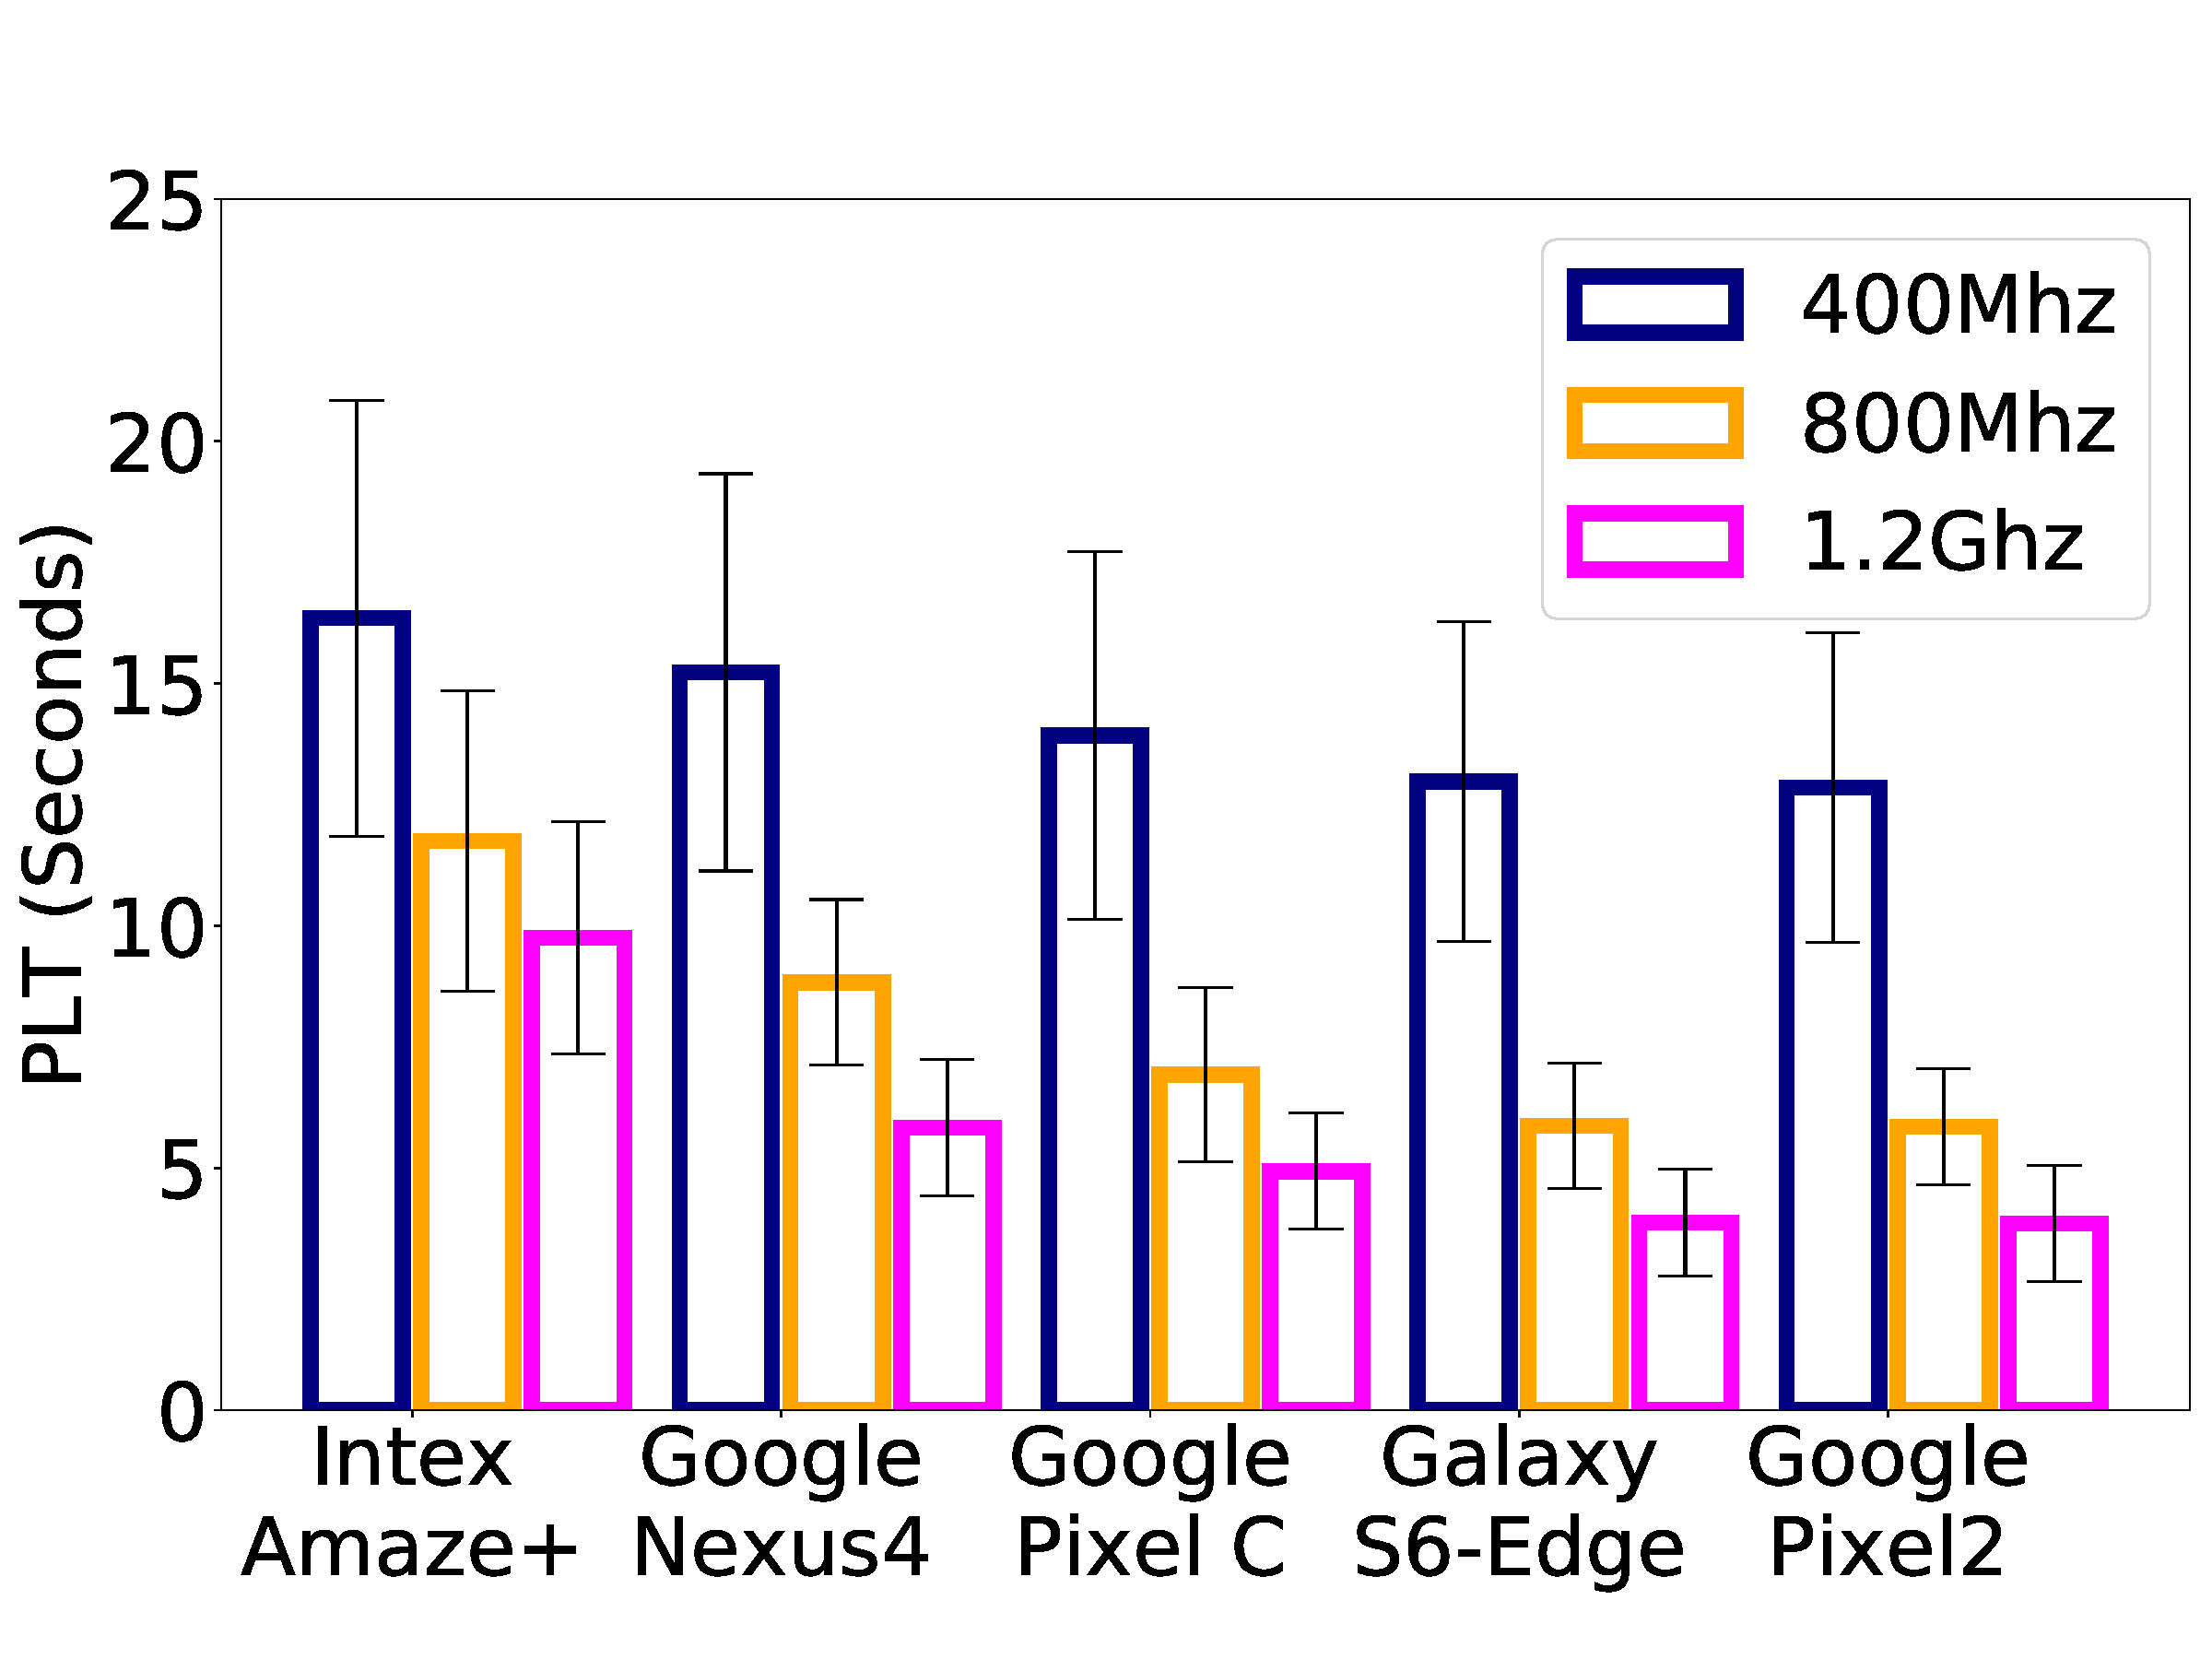
\includegraphics[width=1\linewidth]{sections/device-work/clock-device}
        \caption{Clock}
    \end{subfigure}
    \begin{subfigure}[b]{0.33\textwidth}
        \centering
        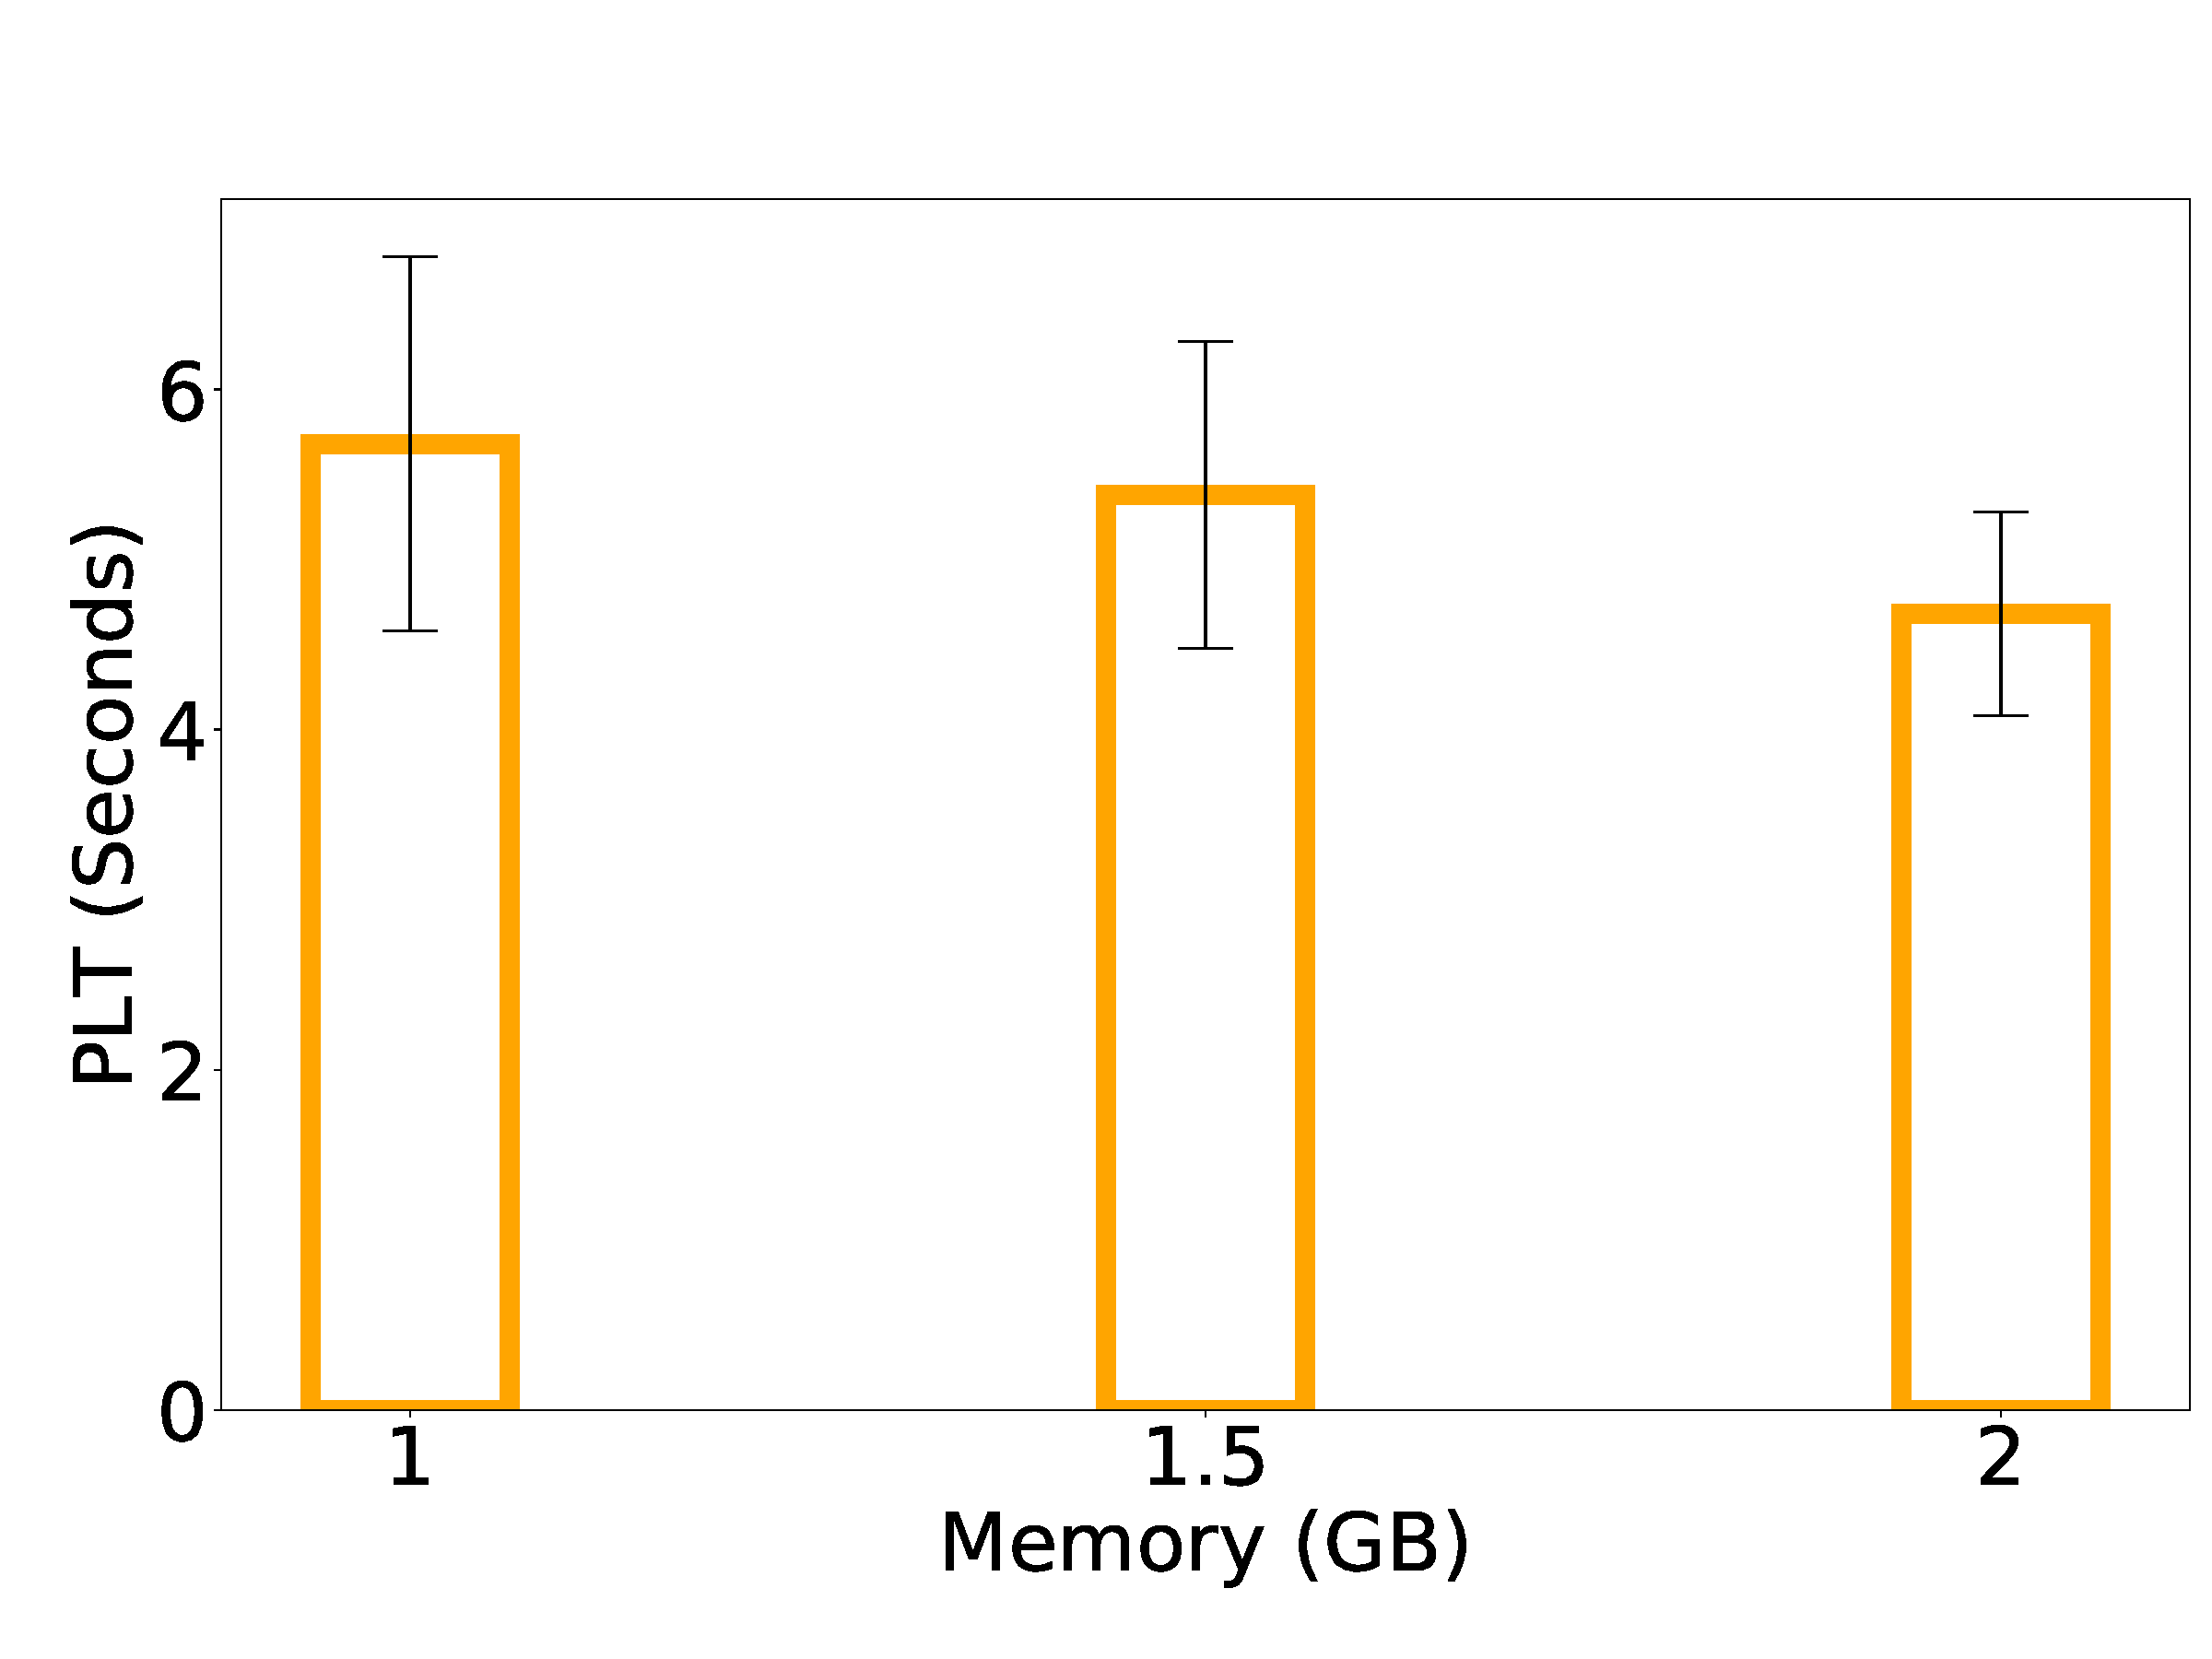
\includegraphics[width=1\linewidth]{sections/device-work/plt-memory}
        \caption{Memory}
    \end{subfigure}%
    \begin{subfigure}[b]{0.33\textwidth}
        \centering
        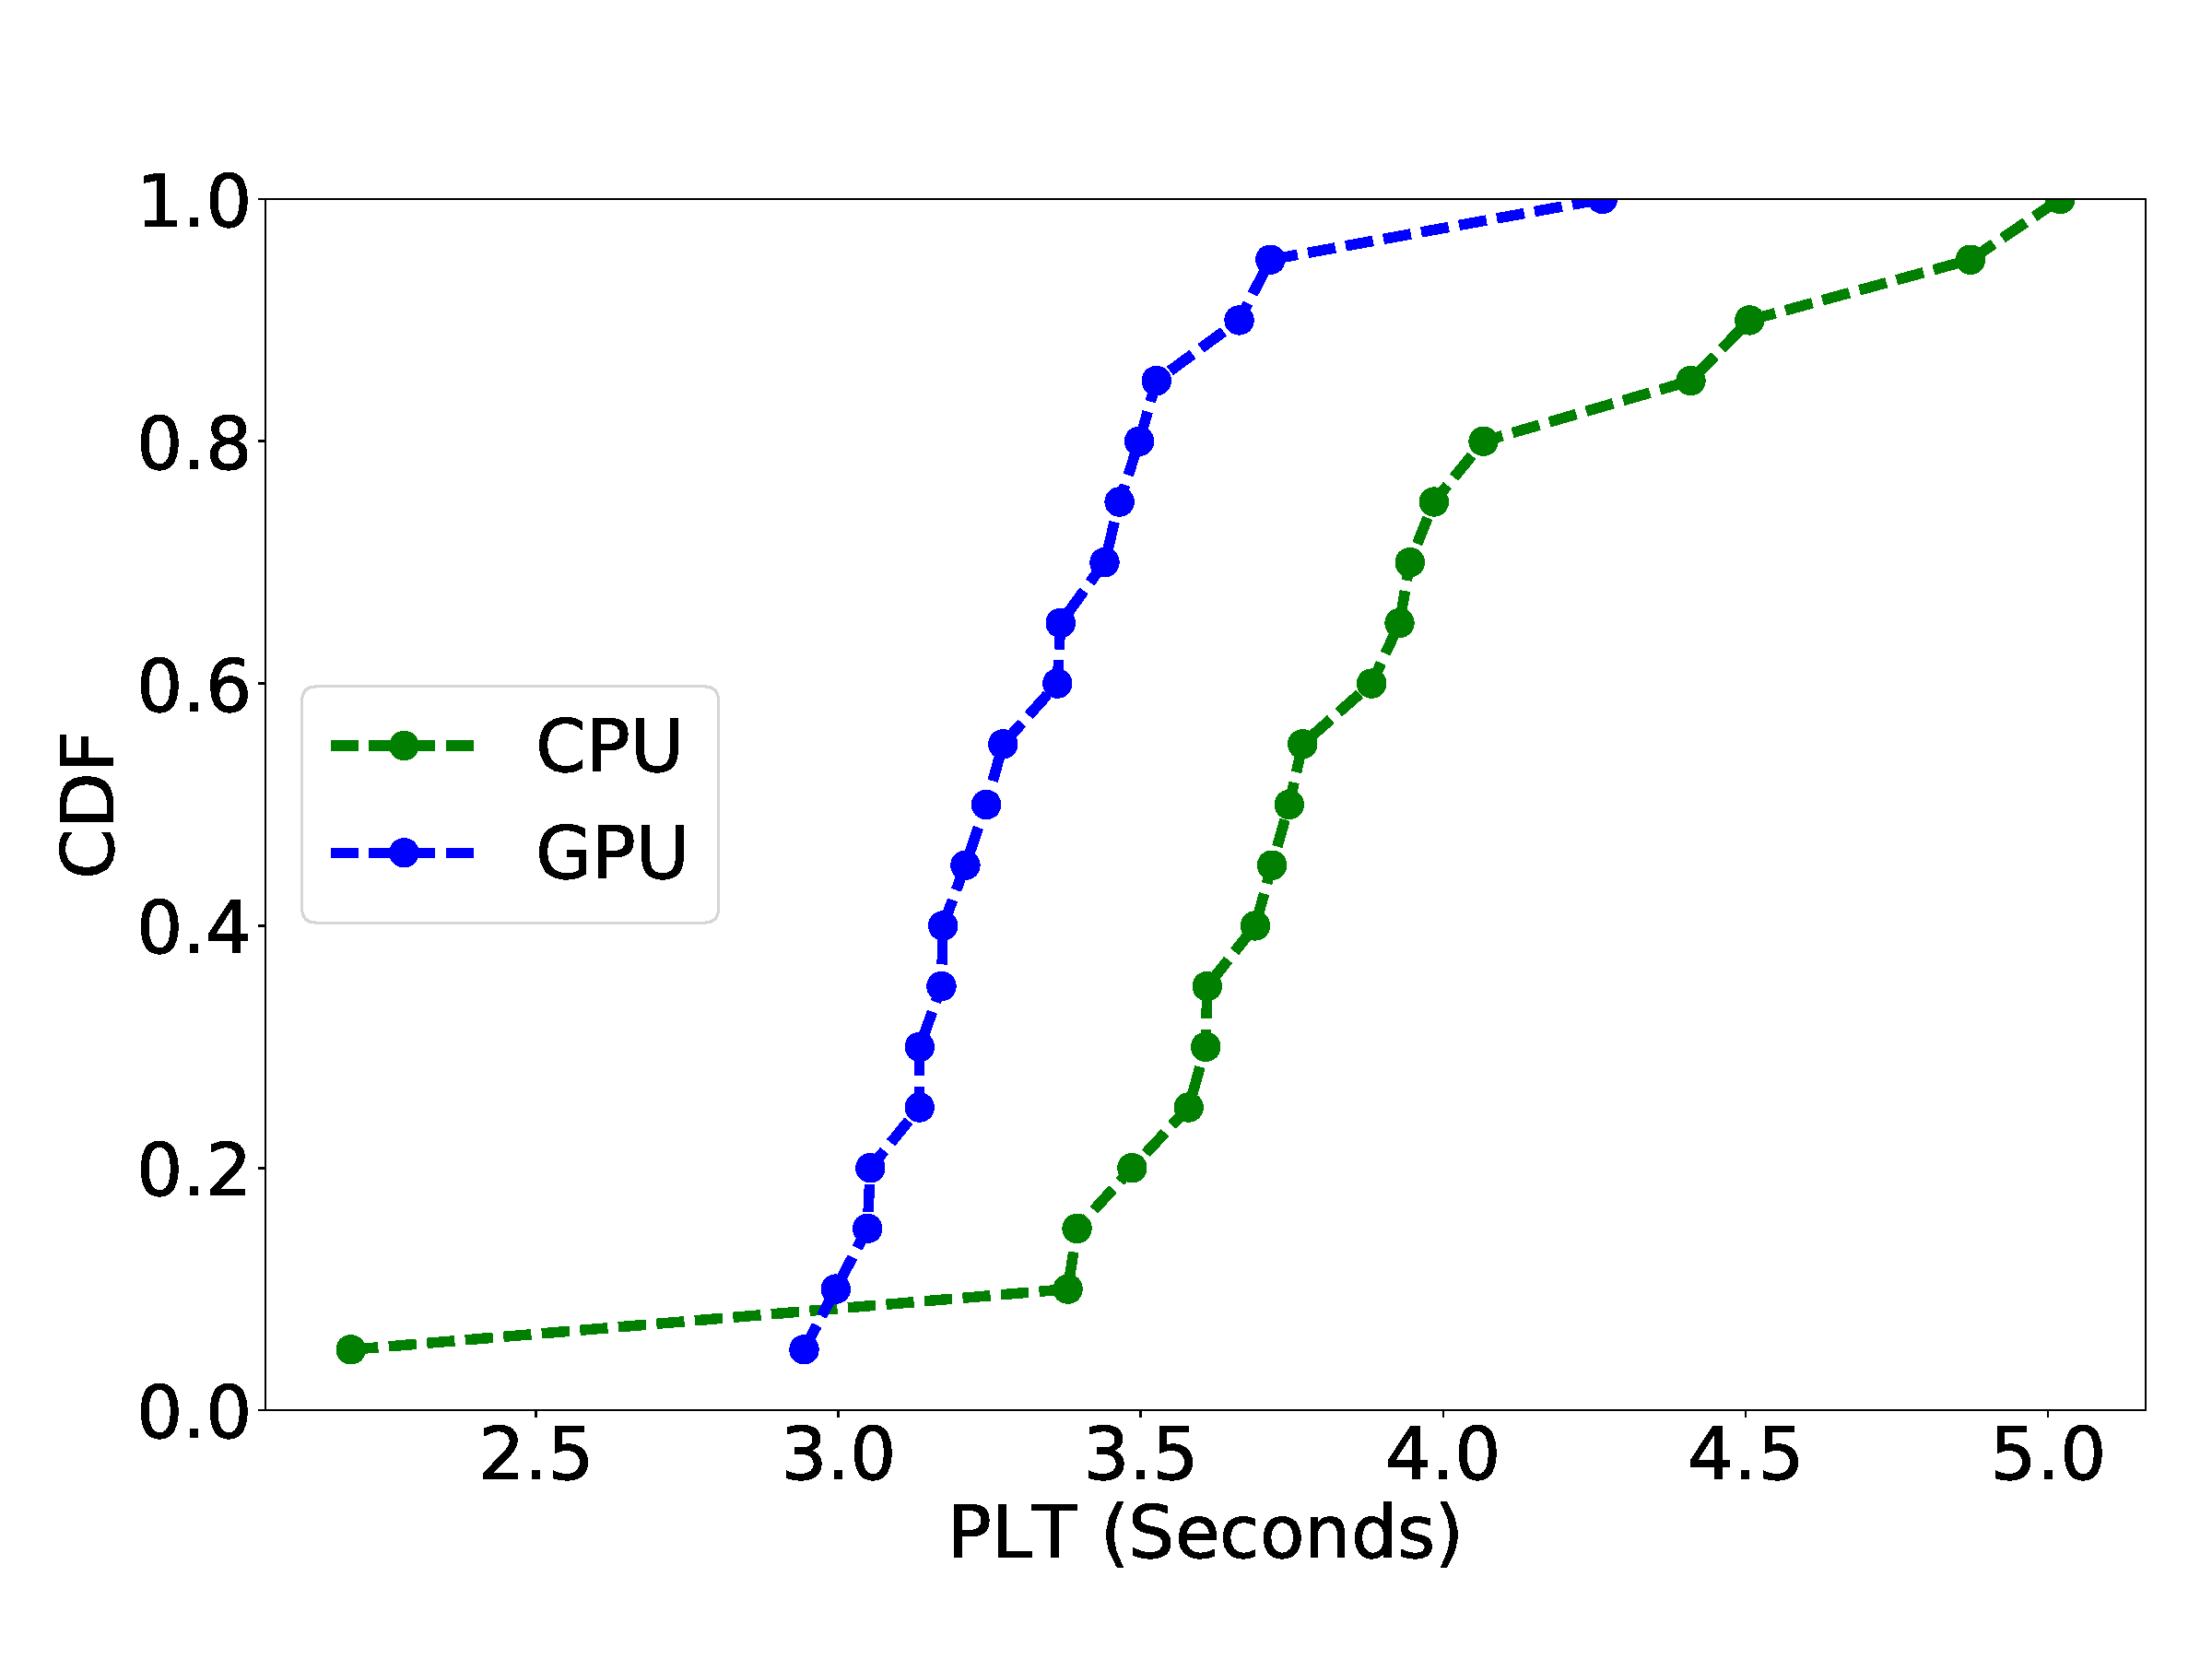
\includegraphics[width=1\linewidth]{sections/device-work/plt-gpu}
        \caption{GPU}
    \end{subfigure}
     \caption{Impact of CPU, memory, and GPU resources on Page Load Time (PLT). Varying the CPU speeds has the most impact on PLT compared to the impact of varying memory availability or leveraging the GPU for rendering. }
     \vspace{-0.2in}
     \label{fig:isolation}
\end{figure*}


\subsection{Measurement Methodology} 
\label{sec:motivation}

As a first step, we study the performance of the three Internet applications---Web browsing, Video streaming, and Video telephony across 7  different smartphones. 
The phones are chosen so that there is a significant
diversity in terms of hardware/OS and cost. Table~\ref{tab:device_types} shows the different devices. The cost ranges from  about \$60 to \$880, and the maximum CPU clock frequencies range from 1300\,MHz to 2457\,MHz. The first two phones in the table, Intex Amaze+ and Gionee F103 are popular phones in India.

We first describe default experimental setup 
before going over to the results.

\subsubsection{Setup}
\label{sec:setup}

%The goal of these initial experiments is to measure the performance of Web, video streaming and telephony, under the same network conditions on the different devices. We use YouTube and Skype, the most popular applications for streaming and telephony respectively. In this section, we first describe the measurement set-up for each of the three applications and compare the QoE performance on different devices.
%All experiments are conducted under default Governors. 

\noindent\textbf{Web Browsing:} We measure browsing performance over Chrome 63.0.3239.111 in terms of Page Load Time (PLT). 
%For Web browsing, the Page Load Time (PLT) metric is used as it gives a holistic view of the different activities that are part of a web page load. 
PLT is the time elapsed between when the URL is sent to the server and when the DOMLoad event is fired~\cite{wang2013demystifying}. We load the top 50 Web pages from the Alexa~\cite{alexa} and estimate the average PLT. We automate the page loads for repeatability using Chrome remote debugging protocol~\cite{ggle} over Android Debug Bridge (ADB)~\cite{adb}.

\noindent\textbf{Video Streaming:} We use {\bf YouTube} to measure video streaming performance using two QoE metrics: {\em start-up latency} and {\em stall ratio}. 
Start-up latency is the time from when the request was issued to when the the application starts displaying frames. Stall ratio is the  amount of time the video stalls during the playback expressed as a fraction
of playback time.
Both of these metrics can be measured using YouTube player APIs~\cite{youtubeapi}. % to capture video playback events such as \textit{video loaded, started, buffering} and \textit{playing}. 
%We log these events during the video playback and measure the QoE metrics from these events.
%
The performance is measured over a 5 minute FullHD format (1080p) video clip. We use ADB~\cite{adb} to programmatically request the video content for repeatability.%\footnote{We use Jimmy Kimmel and Stormy Daniels interview video clip\cite{youvideo}. We use only one video as it does not matter which video(s) to use in our experiments} from YouTube all the experiments.
%We initiate the YouTube video request using Android intents through Android Debug Bridge (ADB) on Linux laptop connected with the phone through USB interface. 

\noindent\textbf{Video telephony:} We use {\bf Skype} to measure performance of video telephony. We measure QoE in terms of {\em frame rate}, a commonly used metric~\cite{yu2014can}.
%For telephony, we use bitrate and framerate QoE metrics.
%Bit rate is the speed at which the video is received and is measured in bits per second. \todo{strange
%definition of video bit rate.} 
Frame rate is measured as the number of frames shown per second and is available from the Skype technical information displayed during the call. Unfortunately, Skype does not provide APIs to extract the frame rate information from this technical information display.
Instead, we screen record~\cite{azscreen} the Skype technical information and extract the frame rate using an optical character recognition tool~\cite{ocr-tesseract}. 

Since Skype is an interactive application, it requires an active participant on both ends. When the Skype call is placed from the mobile to a laptop, the laptop runs a virtual Webcam~\cite{mancam} that plays a video file in Skype instead of camera feed; at the mobile end, the video can be seen during the Skype call. 
We use the same 5 minute video used in YouTube experiments. To automate the Skype call such as starting and ending calls, we use AndroidViewClient (AVC) library \cite{awc}. 

 
%We observe a CPU usage of less than 15\% during screen recording as recording and encoding mostly using GPU, and hence we assume it does not affect our experiments much.
%Unlike YouTube, we have two clients in Skype. One client is placed on a Windows Laptop and the other is placed on phone.

%A User Interface (UI) automation script is created with automated touches using AWC.

%So, whenever our UI automation script places the call on phone, the Windows laptop client receives the call and sends the pre-recorded video instead of camera output.


%The DOMLoad event gets fired when all objects are fetched, processed, and added to the DOM. 
%Alternatively, as our system does not inherently rely upon PLT, the system can be easily adapted to use other web page performance QoE metrics, such as SpeedIndex \cite{spdindex}, which measures when content above the fold is fully loaded, and Klotski \cite{butkiewicz2015klotski} and WebGaze \cite{kelton2017improving} which measure the direct user perception of a web page load. 
%We use Google Chrome's Remote Debugging protocol~\cite{ggle} to trace browser events in measuring PLT. 
%We breakdown PLT into network and compute activities using WProf \cite{wang2013demystifying}.

{\noindent \bf Network Set Up:}
As the focus of this work is to measure the impact of the device hardware, the 
experiments are set up to minimize the impact of the network and the Web/Video servers.
For video streaming and video telephony, we host the videos on a windows laptop on our LAN. 
In case of Web, we host the pages on a desktop on our LAN. The LAN is created using 
an Aruba Access Point (AP) with 72\,Mbps link speed, 10\,ms RTT and 0\% Loss. The mobile device connects to the server over our LAN. We verified that the network performance of the LAN is consistent.  

For each workload, we repeat the experiment 20 times and present the average and standard deviation. During the experiments, the average CPU load is less than 15\%. %\mallesh{We also measure the PLT under different CPU load and clock conditions. We observe a slight increase of 19\% PLT under 100\% load with 1512MHz clock while a significant increase of 86\% PLT under 100\% load with 384Mhz. } \todo{these last sentences in green do not make any sense.}
%\todo{anything about governors?} \mallesh{For governors, I have two datasets. First I have a plot showing the impact of governors on PLT. There are four governors: ondemand, interactive, performance and powersave. Performance has around 3 seconds PLT, interactive and ondemand have around 4 seconds and powersave has 10seconds (because it uses low clock). Do we need this? The second plot that I have shows the clock frequency used by different governors during the pageload. I am not sure if we can motivate by showing this, that the governors change the clock during the application processing, and hence we focus on clock.}

\begin{figure*} [t]
    \begin{subfigure}[b]{0.5\textwidth}
        \centering
        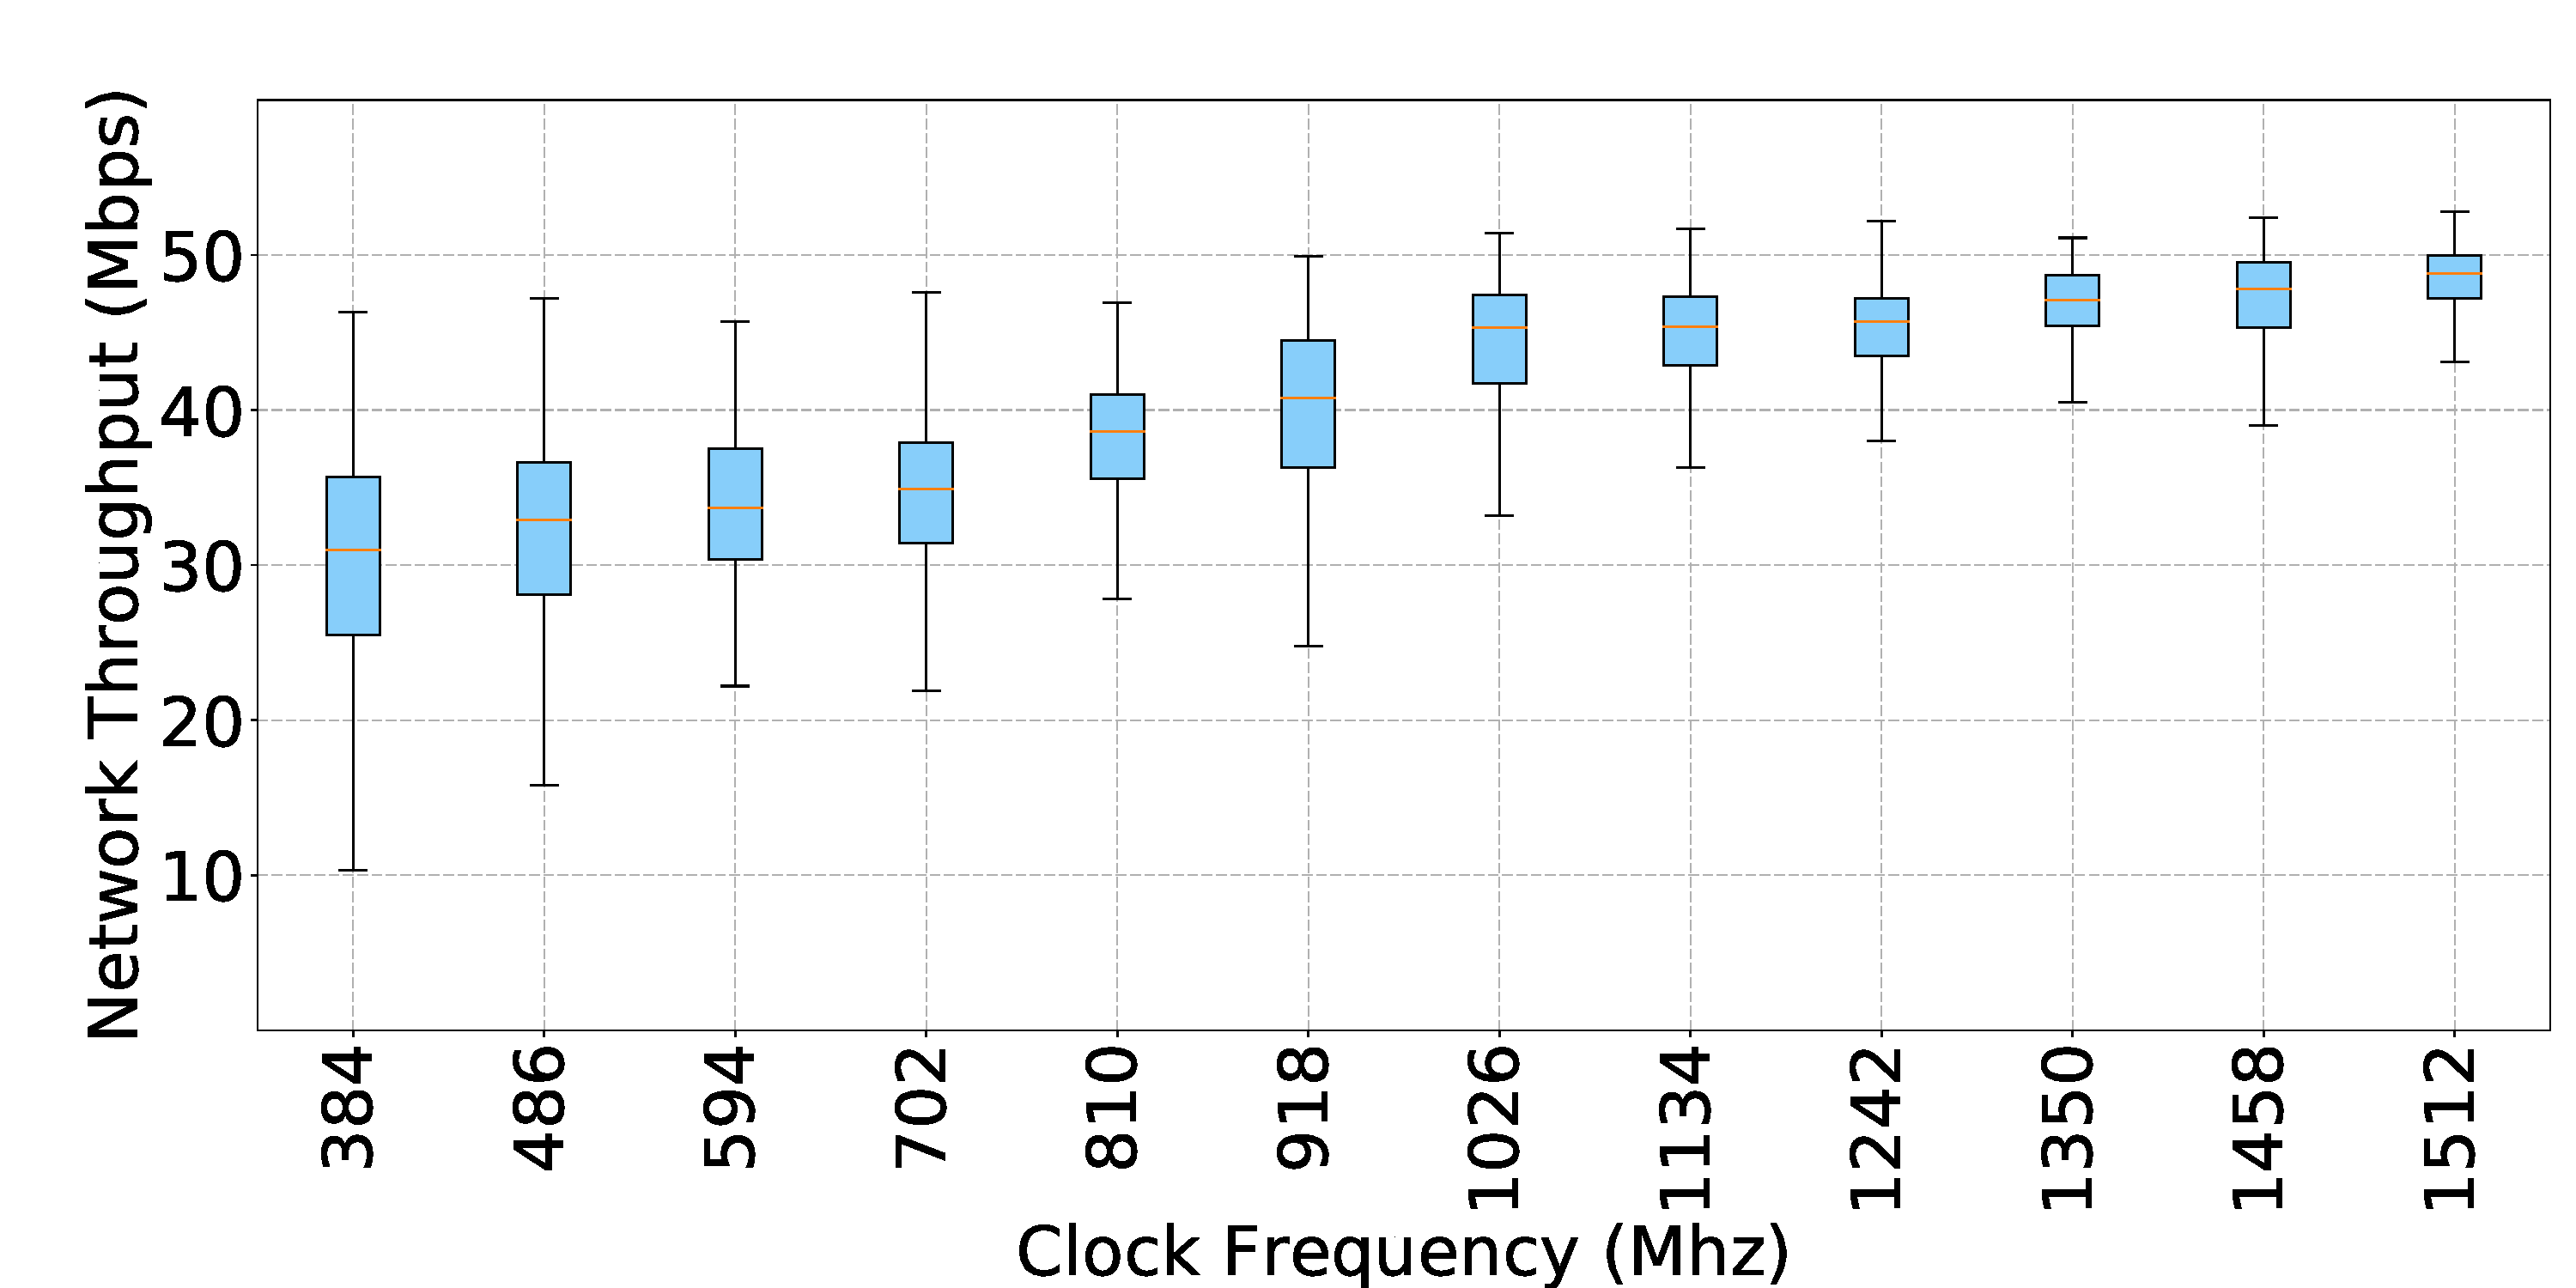
\includegraphics[height=0.5\textwidth,width=1\textwidth]{sections/device-work/Throughput}
        \caption{Throughput vs. Clock}
    \end{subfigure}
    \begin{subfigure}[b]{0.5\textwidth}
        \centering
        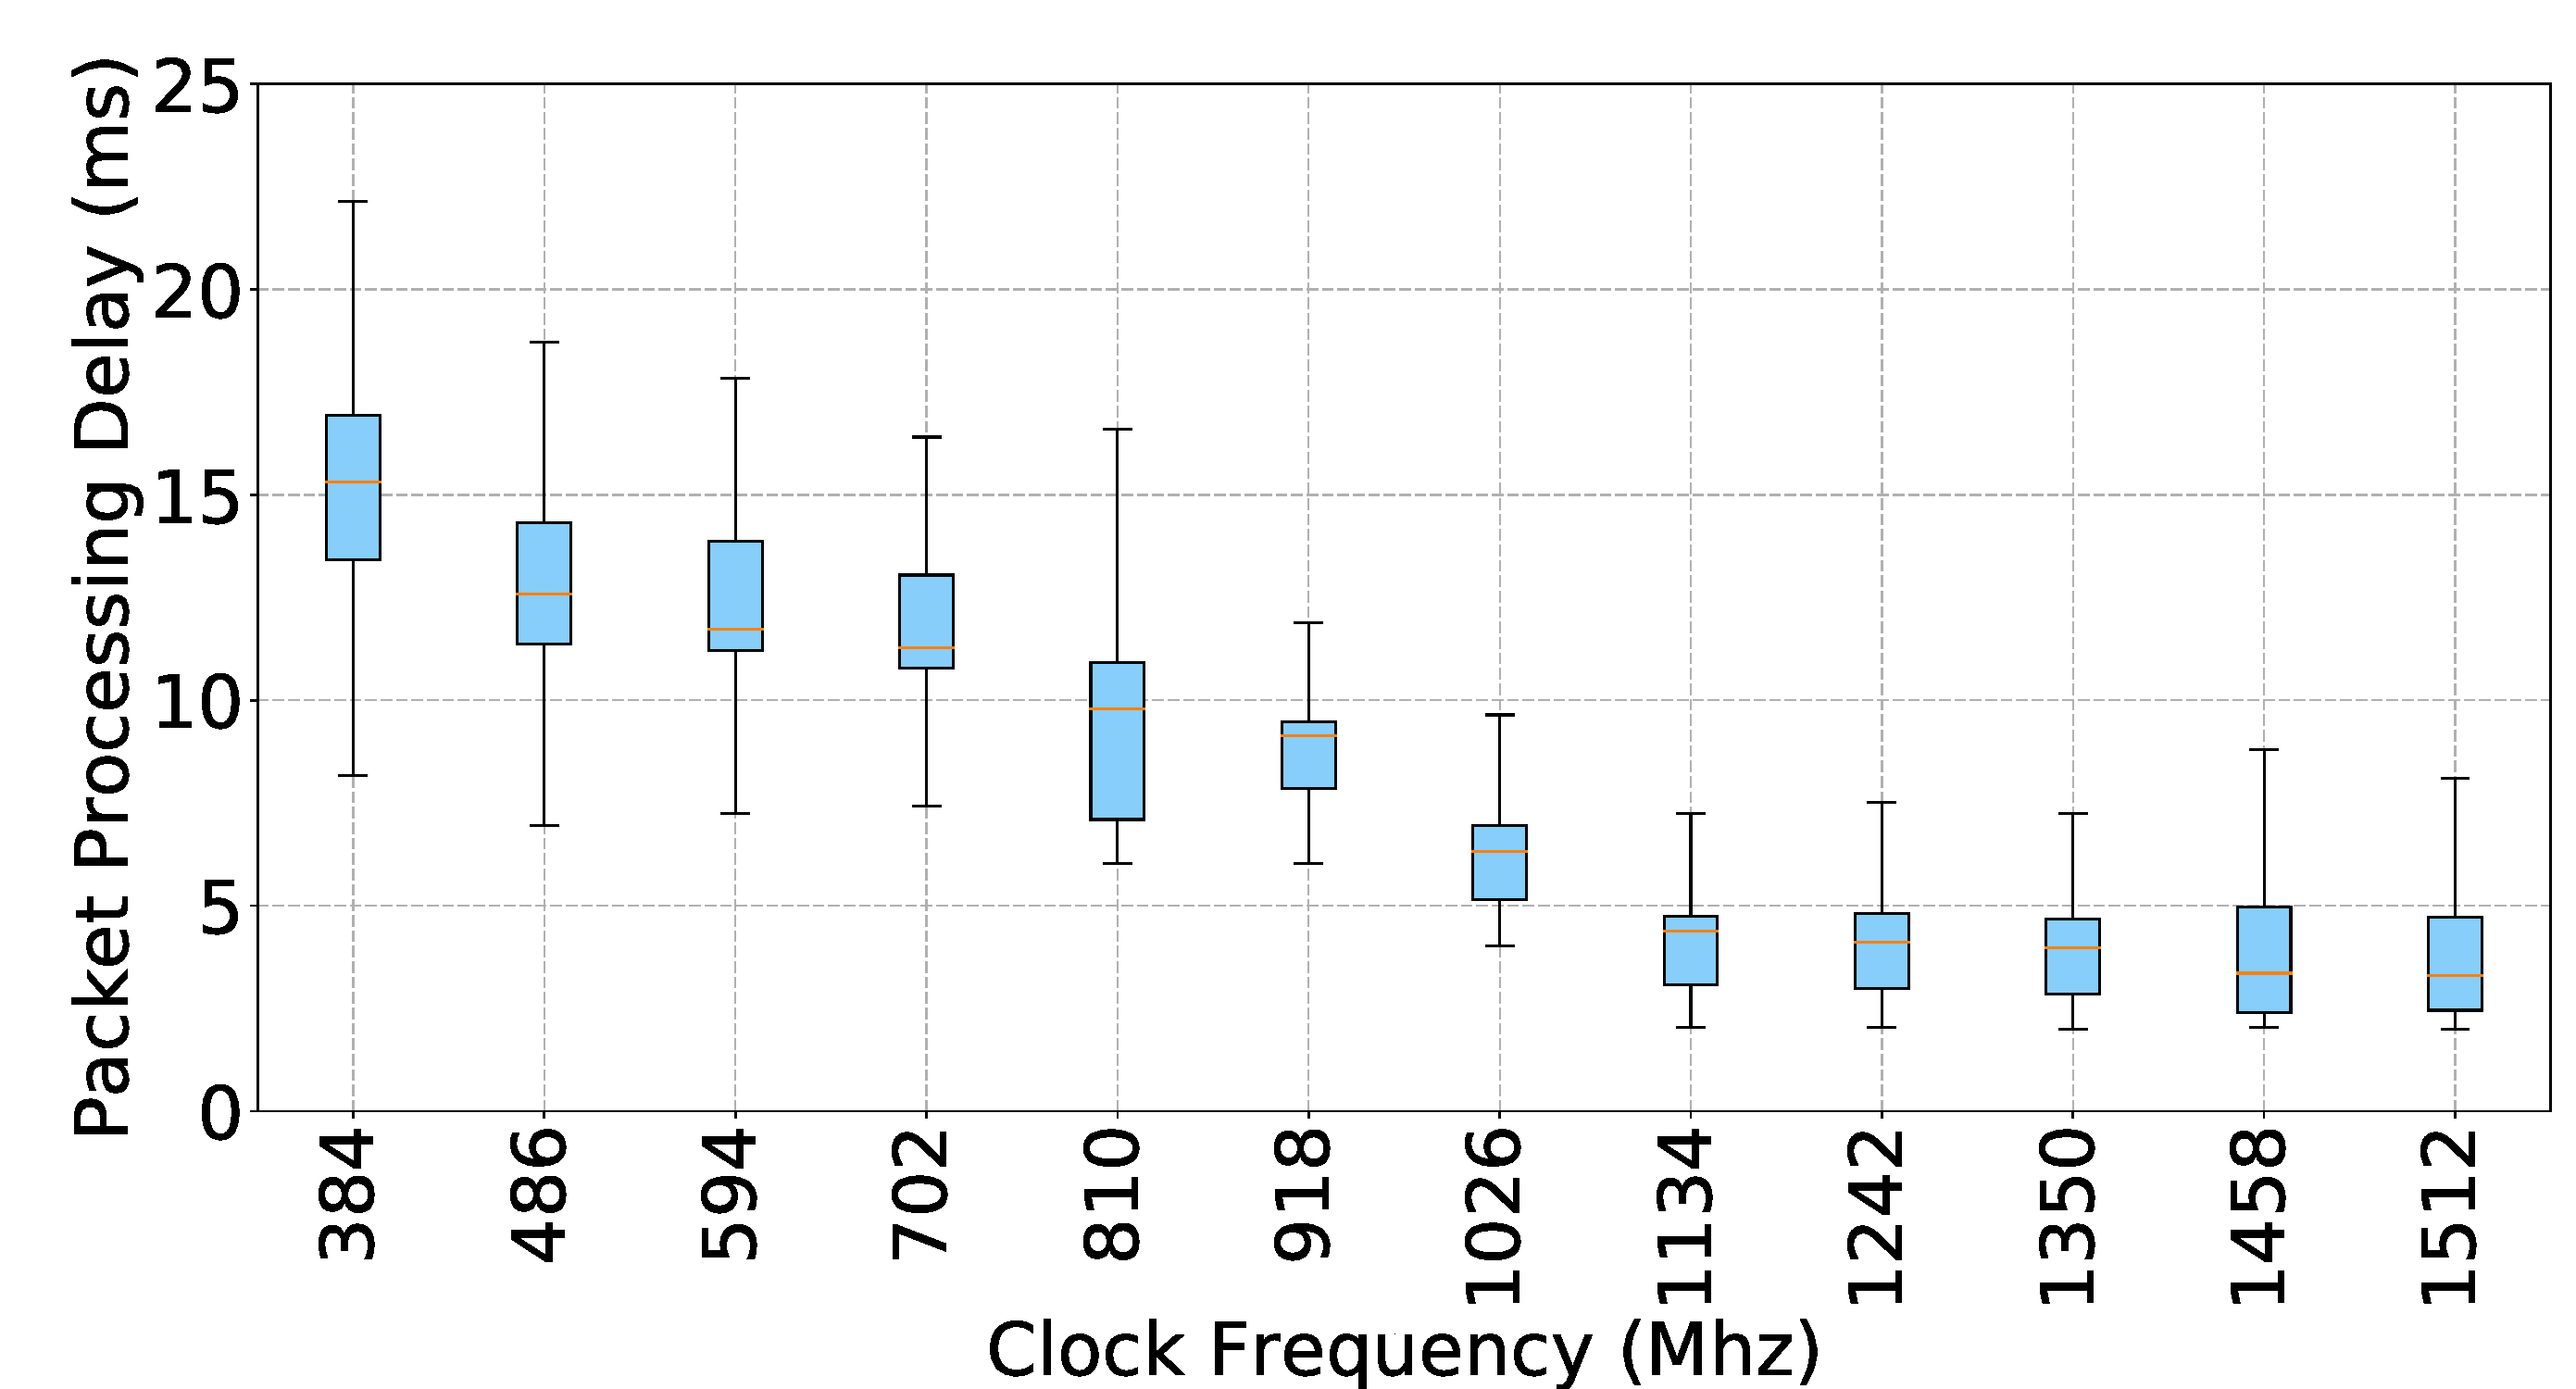
\includegraphics[height=0.5\textwidth,width=1\textwidth]{sections/device-work/ppd}
        \caption{Packet processing delay vs. Clock}
    \end{subfigure}%
     \caption{Second-order effect of CPU speed on network. (a) TCP throughput reduces from an average of 48 Mbps to 32 Mbps under slow clock under the same network conditions, b) The cause for this reduction in throughput is internal to the device; the average TCP packet processing delay increases by 12 ms at slow CPU speeds. Experiments conducted on Nexus 4.}
     \label{fig:tcp-perf}
     \vspace*{-1em}
\end{figure*}


\subsubsection{Application QoE Across Low- and High-end Devices}

Figure \ref{fig:motivation} shows the performance of the three applications across the devices. Based on the device model, there is significant different in performance even though all experiments
are done with the same network conditions. 

For Web loads (Figure \ref{fig:motivation}a), there is a 7 seconds difference in average PLT between the low-end Intex Amaze+ phone and the high-end Google Pixel2. The variance in PLT is also higher ($>$3 seconds) in the Intex Amaze+ compared to Google Pixel 2. This variance must stem from the device itself, since the network conditions are the same.

In the case of YouTube (Figure \ref{fig:motivation}b), there is a linear increase 
in start-up latency from 2 to 5 seconds from the high-end to low-end devices. However, after the start-up latency, there is zero impact on the stall ratio. In effect, once the user waits for the video to start, there is practically no difference in QoE between the low-end and the high-end device. For Skype (Figure \ref{fig:motivation}c), frame rate decreases from 30fps to 18fps between the high- and low-end devices.

For the most part, application QoE is correlated with the device cost.  A
cheaper device provides poorer performance. The only outlier is Pixel2 
which outperforms SG S6-edge despite being less expensive. It, however,
has a better specification. 

The experiments were conducted under the default {\em frequency governor} setting. 
Frequency governors~\cite{ad-governors} on 
Android scales CPU speeds according to power and performance considerations. In the default case, 
Governors set the best CPU speeds according to the load on the CPU and available power. 
The experiments were done with the phones connected to external power so that
power does not impact performance. 
%We find the three applications are behaving very differently on all devices. Web has nonlinear impact, \textit{YouTube} and \textit{Skype} have linear impact.  For video, we see a large gap in performance between \textit{YouTube} and \textit{Skype}. YouTube shows a linear increase in start-up latency from 2 to 5 seconds while Skype has a reduction in framerate of 10 from Pixel2 to Intex phone respectively. However, YouTube only has the start-up effect and shows zero effect of stall ratio across all devices. Although, the start-up latency is varied by more than 3 seconds across devices, the QoE impact while watching the video is zero. This descrepancy can be due to many device parameters such as CPU clock, RAM, hardware accelerators such as GPU, DSP and other application specific hardware chips. 


\subsubsection{Individual Impacts of CPU, Memory and GPU}
\label{sec:impact_cpu}
In this section, we drill down on the device specification that impacts the performance most. Five device specifications in Table~\ref{tab:device_types} can potentially impact application performance---CPU speeds, GPU configuration, memory capacity, OS, and number of cores. Prior work \cite{gao2015study,blake2010evolution} 
has shown that the Internet applications do not typically 
use more than two cores and thus the performance of applications does not change with increase in the number of cores. Also, the OS  does not significantly impact the application performance~\cite{corral2016preserving}. %So, we focus on CPU, memory and GPU parameters only.

Figure~\ref{fig:isolation} shows the impact of the remaining three resources---CPU, memory, and GPU---on Web loads. The experiments are the same as described in \S\ref{sec:setup}. The effect of a given resource is isolated by changing its value while keeping the remaining set up constant. 

The CPU clock frequency is changed using governors~\cite{ad-governors} mentioned before. Figure~\ref{fig:isolation}a shows the effect of CPU clock on 5 different devices.\footnote{The two remaining devices were not tested because changing the CPU clocks required rooting the phone.} 
The CPU clock has significant impact on application performance, improving PLT by an average of 43\% and 71\% 
when going from a slow CPU (400 MHz) to fast CPU (1.2 GHz) on the Intex Amaze+ phone (a low-end phone) and the Google Pixel\,2 (a high-end phone), respectively. In terms of time this is about 6\,seconds 
and 9\,seconds respectively.

Figures~\ref{fig:isolation}b and \ref{fig:isolation}c show that the effect of memory and GPU is much less drastic compared to CPU. These experiments were conducted on the Nexus\,4 phone.
We change memory capacity by creating RAM disks \cite{ramdisks} (in steps of 512MB) from available memory and assigning these RAM disks to the application.  %to memory intensive workloads to occupy completely. We can also create a memory hungry application to occupy the memory directly, but the Android low-memory killers will kill the application. By creating RAM disks, we can divide the RAM into multiple chunks and give it to specific application. 
We use Chrome browser settings to enable or disable  GPU accelerated rendering of a web page. Improving memory availability from 1\,GB to 2\,GB improves PLT  modestly by 17.6\% or about 1\,second. 
The PLT with GPU accelerated page rendering has just 0.5 seconds less than CPU accelerated rendering.  

The key takeaway is that CPU speed has the most impact on Web QoE. We verified this trend in Video streaming and telephony as well; we omit the graphs for brevity. 
Accordingly, in this paper, we focus on the effect of CPU clock on application performance. 


 
